  
\documentclass{beamer}
\usepackage{listings}
\usepackage{graphicx}
\usepackage{epstopdf}
\usepackage{hyperref}

\lstset{
		tabsize=4,
        basicstyle=\scriptsize,
        %upquote=true,
        aboveskip={1.5\baselineskip},
        columns=fixed,
        showstringspaces=false,
        extendedchars=true,
        breaklines=true,
        prebreak = \raisebox{0ex}[0ex][0ex]{\ensuremath{\hookleftarrow}},
		frame=tRBl,
		%frameround=tttf,
		numbers=left,
		numberstyle=\tiny,
		numbersep=5pt,
        showtabs=false,
        showspaces=false,
        showstringspaces=false,
        identifierstyle=\ttfamily,
        keywordstyle=\color[rgb]{0,0,1},
        commentstyle=\color[rgb]{0.133,0.545,0.133},
        stringstyle=\color[rgb]{0.627,0.126,0.941},
        aboveskip=5pt
}

\usetheme{AnnArbor}
\usecolortheme{beaver}
\setbeamertemplate{note page}[plain]
\begin{document}

\title{Client Side and Presentation}
%\subtitle{example using Sinatra}
\author[Konstantinos Karasavvas]{Konstantinos Karasavvas} %\\{\small Software Architect and Engineer}}

%http://www.linkedin.com/pub/konstantinos-karasavvas/14/64b/14b
\institute{CITY College}
\date{\today} 

\begin{frame}
  \titlepage
\end{frame}

\begin{frame}
\setcounter{tocdepth}{1}
\frametitle{Table of contents}
\tableofcontents
\end{frame} 





\section{HTML} 
\begin{frame}[fragile]\frametitle{HTML} 

  \begin{itemize}
    \item HyperText Markup Language
    \begin{itemize}
      \item markup language to define web pages
    \end{itemize}
    \item defines structure and content (.html, .htm)
    \item HTML (SGML)
    \item XHTML (XML)
    \item 4.01 .. 5
    \item Document Object Model (DOM)
  \end{itemize}

  \begin{lstlisting}[language=html, escapechar={^}]
<!DOCTYPE html>
<html>
  <head>
    <title>This is a title</title>
  </head>
  <body>
    <h1>Hello world!</h1>
  </body>
</html>
  \end{lstlisting}
  
\end{frame}




\section{CSS} 
\begin{frame}[fragile]\frametitle{CSS} 

  \begin{itemize}
    \item Cascading Style Sheets
    \begin{itemize}
      \item style sheet language to describe \textbf{how to display} HTML elements 
    \end{itemize}
    \item in \texttt{<style>..</style>} tags or external style sheets (.css)
  \end{itemize}

  \begin{lstlisting}[language=html, escapechar={^}]
<!DOCTYPE html>
<html>
  <head>
    <title>This is a title</title>
    <style>
      h1 {
        text-align:center;
      }
    </style>
  </head>
  <body>
    <h1>Hello world!</h1>
  </body>
</html>
  \end{lstlisting}

\end{frame}




\begin{frame}[fragile]\frametitle{CSS, cont.} 

  \lstinputlisting[language=html]{code/basic.html}

  \lstinputlisting[language=c]{code/basic.css}

\end{frame}





\section{Javascript} 
\begin{frame}[fragile]\frametitle{Javascript} 

  \begin{itemize}
    \item Javascript (JS)
    \begin{itemize}
      \item interpreted programming language
      \item implemented as part of browsers to enable client-side processing
      \item multi-paradigm: OO, imperative, functional
    \end{itemize}
    \item Allows web page to interact with user directly
    \begin{itemize}
      \item without another client-server round-trip
    \end{itemize}
    \item Can manipulate the DOM
    \item Server-side processing (Node.js)
  \end{itemize}
  
\end{frame}



\begin{frame}[fragile]\frametitle{Javascript, cont.} 

  \lstinputlisting[language=html]{code/basic2.html}

\end{frame}



\begin{frame}[fragile]\frametitle{Javascript, cont.} 

  \lstinputlisting[language=html]{code/basic3.html}

  \lstinputlisting[language=html]{code/basic.js}

\end{frame}




\section{AJAX} 
\begin{frame}[fragile]\frametitle{AJAX} 

  \begin{itemize}
    \item Asynchronous JavaScript and XML
    \begin{itemize}
      \item enables communication with the server in the background
      \item group of technologies: HTML, CSS, DOM, XML, JSON
    \end{itemize}
    \item Typically \textit{JSON} is used
    \item Requests need not be \textit{asynchronous}
    \item Javascript \texttt{XMLHttpRequest} object
  \end{itemize}
  
  \begin{lstlisting}[language=java, escapechar={^}]
// This is the client side
// Initialize the Ajax request
var xhr = XMLHttpRequest();
xhr.open('get', 'send-ajax-data.txt', false);
 
// Send the request to send-ajax-data.php
xhr.send(null);
 
var response = xhr.responseText;
 
alert(response); // 'This is the returned text.'
  \end{lstlisting}
\end{frame}





\section{More CSS} 
\subsection{SASS}
\begin{frame}[fragile]\frametitle{More CSS: SASS} 

  \begin{itemize}
    \item Syntactically Awesome Stylesheets
    \begin{itemize}
      \item CSS metalanguage; scripting language that is interpreted into CSS
    \end{itemize}
    \item CSS deficiencies:
    \begin{itemize}
      \item no variables: colour \texttt{\#ffcc33} needs to be repeated
      \item code blocks cannot be nested (although logical nesting is allowed)
      \item no mixin support: repeated code blocks needs to be repeated in every location
      \item ...
    \end{itemize}     
    \item Two syntaxes
    \begin{itemize}
      \item the indented syntax; haml-like (.sass)
      \item SCSS: the newer syntax; CSS block formatting (.scss)
    \end{itemize}
  \end{itemize}

\end{frame}



\begin{frame}[fragile]\frametitle{More CSS: SASS, cont.} 

  \begin{lstlisting}[language=java, escapechar={^}]
$ gem install sass
$ sass style.scss style.css
  \end{lstlisting}
  
  \begin{columns}[c] 

    \begin{column}{5.5cm}
      \lstinputlisting[language=java]{code/style.scss}
    \end{column}  

    \begin{column}{5.5cm}
      \lstinputlisting[language=java]{code/style.css}
    \end{column}    
    
  \end{columns}
  
\end{frame}



\subsection{LESS}
\begin{frame}[fragile]\frametitle{More CSS: LESS} 

  \begin{itemize}
    \item LESS: metalanguage that is interpreted into CSS
    \item Similar to SASS
    \begin{itemize}
      \item main difference is that real-time compilation can be accomplished via \texttt{LESS.js}
    \end{itemize}
    \item Current implementation is in Javascript
    \begin{itemize}
      \item Can run on both the server (Node.js) and the client (browsers)
      \item Prerequisites: Node.js and NPM (Node Package Manager)
    \end{itemize}
  \end{itemize}

\end{frame}



\section{More Javascript} 
\begin{frame}[fragile]\frametitle{More Javascript} 

  \begin{itemize}
    \item jQuery
    \begin{itemize}
      \item cross-browser Javascript library
      \item easier client-side scripting
      \begin{itemize}
        \item document navigation
        \item DOM element selection
        \item event handling
        \item animations
        \item AJAX
      \end{itemize}
    \end{itemize}
    \item Jquery Mobile
    \item Prototype
    \item ...
  \end{itemize}
\end{frame}




\begin{frame}[fragile]\frametitle{More Javascript: jQuery Example} 

  \lstinputlisting[language=html]{code/jquery.html}

\end{frame}



\subsection{More Javascript: CoffeeScript} 
\begin{frame}[fragile]\frametitle{More Javascript: CoffeeScript} 

  \begin{itemize}
    \item Is an alternative syntax for Javascript
    \item Compiles to Javascript
    \item Offers syntactic sugar
    \item Is indentation-based -- no curly braces
    \item 2/3 lines of equivalent JS file
  \end{itemize}

  \begin{columns}[c]
  
    \begin{column}{5.5cm}
      \begin{lstlisting}[language=java, escapechar={^}]
$ -> 
  $("body").html "Hello!"
      \end{lstlisting}
    \end{column}

    \begin{column}{5.5cm}
      \begin{lstlisting}[language=java, escapechar={^}]
$(function() {
  $("body").html("Hello!");
})
      \end{lstlisting}
    \end{column}

  \end{columns}

  \begin{itemize}
    \item Dart (by Google)
  \end{itemize}

\end{frame}



\subsection{More Javascript: Web Application Frameworks} 
\begin{frame}[fragile]\frametitle{More Javascript: Web Application Frameworks} 

  \begin{itemize}
    \item Web Application Frameworks
    \begin{itemize}
      \item Angular
      \item Ember
      \item YUI
      \item Dojo
      \item ExtJS
      \item Meteor
      \item ...
    \end{itemize}
  \end{itemize}

\end{frame}




\section{Single-Page Applications} 
\subsection{Introduction}
\begin{frame}[fragile]\frametitle{Single-Page Applications} 

  \begin{itemize}
    \item Up and coming
    \item Server
    \begin{itemize}
      \item API (REST)
      \item models, DB, migrations, etc.
      \item but \textbf{no} views
    \end{itemize}
    \item Client
    \begin{itemize}
      \item templates for views
      \item models for updating the views
      \item \textit{controllers}
      \item MV*
    \end{itemize}
    
  \end{itemize}

\end{frame}




\subsection{MVC -- MV*} 
\begin{frame}[fragile]\frametitle{MVC -- MV*} 

  \begin{columns}[c] 

    \begin{column}{6cm}
      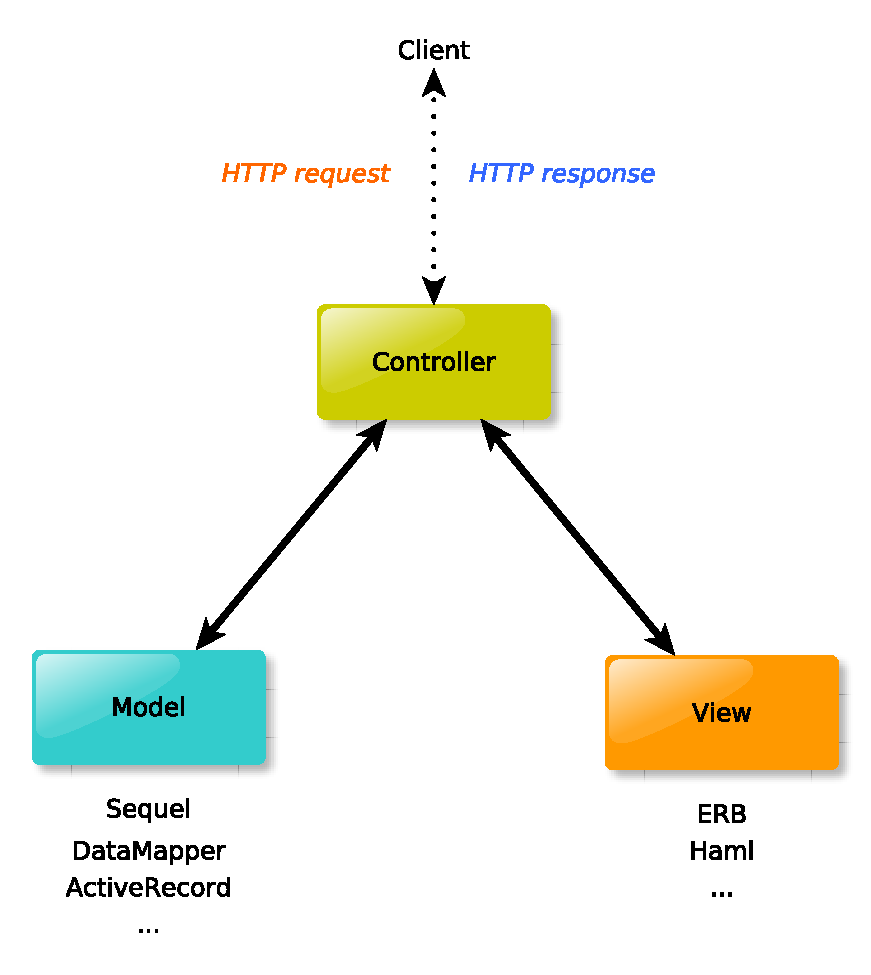
\includegraphics[scale=0.40]{diagrams/mvc.pdf}  
    \end{column}

    \begin{column}{4cm}
      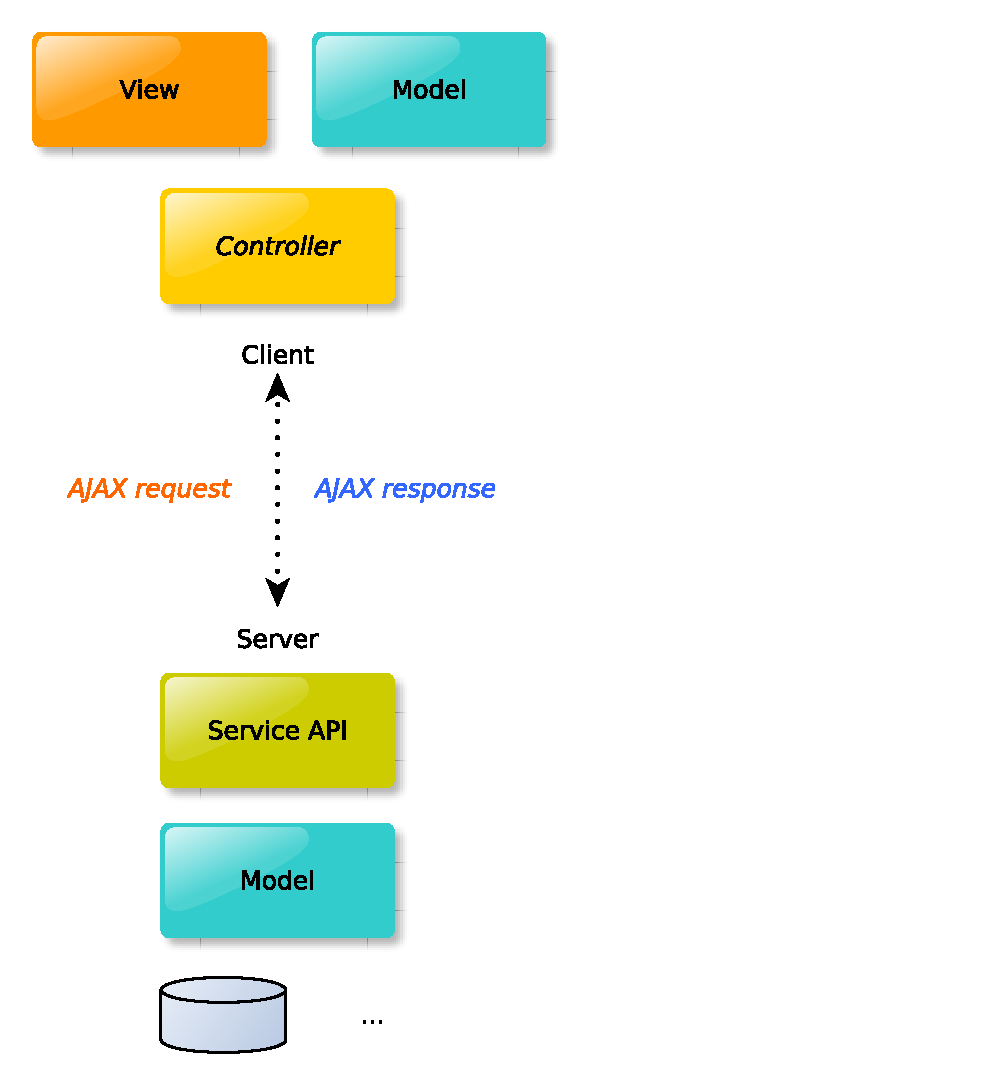
\includegraphics[scale=0.40]{diagrams/spa_mvc.pdf}  
    \end{column}

  \end{columns}

\end{frame}




\subsection{AngularJS}
\begin{frame}[fragile]\frametitle{AngularJS: why?} 
  
  \begin{itemize}
    \item Backed by Google
    \item Actively maintained
    \item Comprehensive feature set
    \item It doesn't get in the way
    \item Large and quickly growing community
    \item Built for testability
    \item Get started in minutes
    \item Built with REST in mind
    \item Fast
  \end{itemize}

\end{frame}




\begin{frame}[fragile]\frametitle{AngularJS: Introduction} 
  
  \begin{itemize}
    \item Features:
    \begin{itemize}
      \item Client-side MV\textit{C}
      \item Templating
      \item Two way data-binding
      \item Routing
      \item Event dispatching
      \item Extensibility
      \item Dependency Injection
    \end{itemize}
  \end{itemize}
\end{frame}



\begin{frame}[fragile]\frametitle{AngularJS: Example 1} 

  \lstinputlisting[language=html]{code/angular/hello.html}
  
\end{frame}




\begin{frame}[fragile]\frametitle{AngularJS: Example 1, cont.} 

  \begin{center}
    \includegraphics[scale=0.50]{images/hello_angular.png}    
  \end{center}

\end{frame}




\begin{frame}[fragile]\frametitle{AngularJS: Example 2} 

  \lstinputlisting[language=html]{code/angular/repeat_angular.html}
  
\end{frame}




\begin{frame}[fragile]\frametitle{AngularJS: Example 2, cont.} 

  \lstinputlisting[language=html]{code/angular/controllers/names.js}

\end{frame}




\begin{frame}[fragile]\frametitle{AngularJS: Example 2, cont.} 

  \begin{center}
    \includegraphics[scale=0.50]{images/repeat_angular.png}    
  \end{center}

\end{frame}





\section{Web Design}
\subsection{Introduction}
\begin{frame}[fragile]\frametitle{Web Design} 

  \begin{itemize}
    \item ... is an art
    \item Requires a whole different expertise
    \begin{itemize}
      \item not just HTML, CSS and Javascript
    \end{itemize}
    \item Which colours look good combined?
    \item What button sizes?
    \item How to layout our application?
    \item How to make menus? Vertical? Horizontal?
    \item Device heterogeneity? Responsive design?
    \item Cross-browser?
    \item Consistency?
    \item Images?
    \item Fortunately, there are tools to help
  \end{itemize}

\end{frame}

% http://modernizr.com/docs/
% tool that falls back ti polyfills (JS) when something is not 
% supported in a browser

\subsection{Front-end Frameworks}
\begin{frame}[fragile]\frametitle{Front-end Frameworks: Easier web development!} 

  \begin{itemize}
    \item Twitter Bootstrap
    \item Foundation
    \item GroundworkCSS
    \item Gubmy
    \item HTML KickStart
    \item Kube
    \item Bootmetro
    \item Bootstrap-based
    \begin{itemize}
      \item Fbootstrapp
      \item Kickscrap
      \item FlatUI 
    \end{itemize}
  \end{itemize}

\end{frame}




\subsection{Twitter Bootstrap}
\begin{frame}[fragile]\frametitle{Twitter Bootstrap} 

  \begin{itemize}
    \item Developed by Twitter's developers
    \item Features:
    \begin{itemize}
      \item \textbf{Grid system} with support for \textbf{Responsive Design}
      \item \textbf{CSS classes} for buttons, forms, tables, icons, navigation bars, labels, progress bars, etc.
      \item \textbf{Javascript UI widgets} for modals, menu dropdowns, images slider, accordions, notifications, etc.
    \end{itemize}
    \item Highly customizable using LESS
  \end{itemize}

\end{frame}




\begin{frame}[fragile]\frametitle{Twitter Bootstrap: Example} 

  \includegraphics[scale=0.28]{images/bootstrap_demo.png} 

\end{frame}




% how can client talk to server?? how can JS talk to server?
% how server can talk to client? websockets?




\end{document}
